%================================================================================================
% Lemma 4.5
%================================================================================================
\begin{sublemma}\label{lemma4.5}
Assume $g$ is a connected graph. Forall node $v \in explored_{n+1}$:
\begin{enumerate}
  \item $dist_{n+1}[v] < \infty$
  \item $dist_{n+1}[v]  \leq \delta(v')$, $\forall v' \in unexplored_{n+1}$.
  \item $dist_{n+1}[v] = \delta(v)$
\end{enumerate}
\end{sublemma}

\begin{proof}
We will prove \texttt{Lemma 4.5} by inducting on the number of iterations. 
\\\\
Let P(n) be: For a connected graph $g$, for $n \geq 1$, forall node $w \in explored_{n+1}$: (L1) $dist_{n+1}[w] < \infty$; (L2) $dist_{n+1}[w] \leq \delta(w')$, $\forall w' \in unexplored_{n+1}$; (L3) $dist_{n+1}[w] = \delta(w)$. 

\paragraph*{Base Case}: We shall show P(1) holds \\
Based on the algorithm, during the first iteration, the node with minimum distance value is the source node $s$ with $dist_1[s] = 0$. Hence during the first iteration, only $s$ is removed from $unexplored_1$ and added to $explored_2$. Since $dist_2[s] = 0 < \infty$, then (L1) holds for P(1). Since all edge weights are non-negative, then the shortest distance value from $s$ to $s$ is indeed $0$, hence $dist_2[s] = 0 = \delta(s)$ and $dist_2[s] \leq \delta(v')$, $\forall v' \in unexplored_2$. Thus (L2) and (L3) holds for P(1). Hence P(1) holds.

\paragraph*{Induction Hypothesis}: Suppose P(i) is true for all $1 \leq i \leq k$. That is, forall $1 < i \leq k$, forall node $w \in explored_{i+1}$: (L1) $dist_{i+1}[w] < \infty$; (L2) $dist_{i+1}[w] \leq \delta(w')$, $\forall w' \in unexplored_{i+1}$; (L3) $dist_{i+1}[w] = \delta(w)$; 

\paragraph*{Inductive Step}: We shall show P(k+1) holds. That is, forall node $w \in explored_{k+2}$, (L1) $dist_{k+2}[w] \neq \infty$; (L2) $dist_{k+2}[w]\leq \delta(w')$, $\forall w' \in unexplored_{k+2}$; (L3) $dist_{k+2}[w] = \delta(w)$;
\\\\
Suppose $u_{k+1}$ is the node added into $explored$ during the $(k+1)^{th}$ iteration, then $explored_{k+2} = explored_{k+1} \cup \{u_{k+1}\}$. We will show that (L1)(L2) and (L3) holds for all nodes in $explored_{k+1}$ in \texttt{Part (a)}, and \texttt{Part (b)} proves (L1)(L2)(L3) holds for $u_{k+1}$, so that the statements holds forall nodes in $explored_{k+2}$. 
\begin{itemize}
  %================================================================================================
  % Lemma 4.5 part (a)
  %================================================================================================
  \item Part(a): \texttt{WTP: After the $(k+1)^{th}$ iteration, $\forall w \in explored_{k+1}$, (L1)(L2)(L3) holds.} 
  \\\\
  Consider each node $q \in (explored_{k+1} \cap explored_{k+2}) = explored_{k+1}$, $q$ must be explored before the $(k+1)^{th}$ iteration. Suppose $q$ is explored during the $i^{th}$ iteration for some $i < k+1$, then based on our induction hypothesis, $dist_{i+1}[q] = \delta(q)$, and $\delta(q) \leq \delta(q'), \forall q' \in unexplored_{i+1}$. 
  \\\\
  \texttt{Proof of (L3)}: Since for each node $q \in explored_{k+1}$, the induction hypothesis implies that $dist_{k+1}[q] = \delta(q)$, then \texttt{Lemma 3.3} imples that $dist_{k+2}[q] = dist_{k+1}[q] = \delta(q)$. (L3) holds for $explored_{k+1}$.
  \\\\
  \texttt{Proof of (L2)}: Based on the algorithm, for each iteration, the algorithm explores exactly one node and never revisits any explored nodes. For each node $q \in explored_{k+1}$ mentioned above, since $q$ is explored before the $(k+1)^{th}$ iteration, then $unexplored_{k+1} \subseteq unexplored_{i+1}$. Since $\delta(q) \leq \delta(q'), \forall q' \in unexplored_{i+1}$, and $unexplored_{i+1}$ includes all node in $unexplored_{k+1}$, then $\delta(q) \leq \delta(q'), \forall q' \in unexplored_{k+1}$. Since proof of (L3) above shows that $dist_{k+2}[q] = \delta(q)$, then $dist_{k+2}[q] \leq \delta(q'), \forall q' \in unexplored_{k+1}$. (L2) holds for $explored_{k+1}$. 
  \\\\
  \texttt{Proof of (L1)}: Since the induction hypothesis implies that $\forall q \in explored_{k+1}, dist_{k+1}[q] < \infty$, and the proof of (L3) above shows that $dist_{k+2}[q] = dist_{k+1}[q]$, then $dist_{k+2}[q] < \infty$. (L1) holds for $explored_{k+1}$.
  \\\\
  Hence we have proved that both (1) and (2) holds for all nodes in $explored_{k+1}$.

  %================================================================================================
  % Lemma 4.5 part (b)
  %================================================================================================
  \item Part(b): (L1)(L2)(L3) holds for $\{u_{k+1}\}$. 
  \\
  Specifically, we want to show: (L1) $dist_{k+2}[u_{k+1}] < \infty$; (L2) $dist_{k+2}[u_{k+1}] \leq \delta(v')$, $\forall v' \in unexplored_{k+2}$, and (L2) $dist_{k+2}[u_{k+1}] = \delta(u_{k+1})$. 


  \begin{enumerate}
  \item (L1) $dist_{k+2}[u_{k+1}] \neq \infty$
  \\
  Since $g$ is a connected graph, then $s$ must have a path to $u_{k+1}$. Since $u_{k+1}$ is the node currently being explored, then we know there must exists a $s-u_{k+1}$ path, denote as $p(s, u_{k+1})$, such any node proceeding $u_{k+1}$ in $p(s, u_{k+1})$ are explored before $u_{k+1}$, i.e., in $explored_{k+1}$. 
  \\
  Denote the node right before $u_{k+1}$ in $p(s, u_{k+1})$ as $u'$, $u' \in explored_{k+1}$. Suppose $u'$ is explored during the $i^{th}$ iteration, $i < k+1$. The induction hypothesis implies that $dist_{i+1}[u'] < \infty$. Since $dist_{i+1}[u'] = min(dist_i[u'], dist_i[u'] + weight(u', u')) = min(dist_i[u'], dist_i[u'] + \infty) = dist_i[u']$, then $ dist_i[u'] < \infty$. \texttt{Lemma 4.4} implies $dist_{k+2}[u_{k+1}] \leq dist_i[u'] + weight(u', u_{k+1}]$, then it follows that $dist_{k+1}[u_{k+1}] < \infty$. (L1) holds for $u_{k+1}$. 
  \\
  \item (L2) $dist_{k+2}[u_{k+1}] \leq \delta(v')$, $\forall v' \in unexplored_{k+2}$
  \\\\
  We will prove (L2) by contradiction. Suppose there exists $w \in unexplored_{k+2}$, such that $dist_{k+2}[u_{k+1}] > \delta(w)$([E4.5.1]). 
  \\
  Consider the shortest path $\Delta(s, w)$ from $s$ to $w$, $\delta(w) = length(\Delta(s, w))$. Since $w \notin explored_{k+2}$, then there must exists some node in $\Delta(s, w)$ that are not in $explored_{k+2}$. Suppose the first node along $\Delta(s, w)$ that is not in the $explored_{k+2}$ list is $w_2$, and the node right before $w_2$ in the $s$ to $w_2$ subpath is $w_1$, thus $w_1 \in explored_{k+2}$. Figure \ref{figure1} below illustrates this construction. 
  
  \begin{figure}[H]
    \centering
    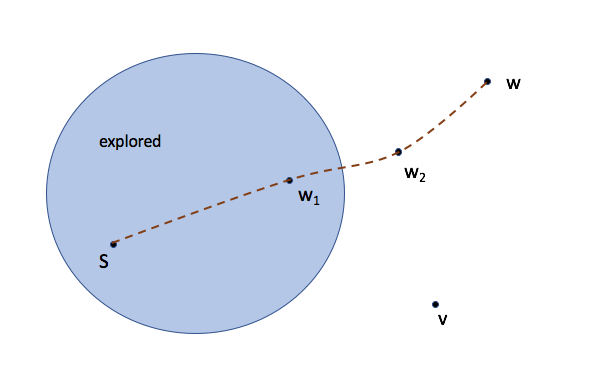
\includegraphics[scale = 0.55]{./figure/pic_proof.png}
    \caption{Lemma 4.5 Proof Construction}
    \label{figure1}
  \end{figure}
  \tab\\
  Denote the subpath from $s$ to $w_1$ in $\Delta(s, w)$ as $p(s, w_1)$, subpath from $s$ to $w_2$ in $\Delta(s, w)$ as $p(s, w_2)$, and subpath $w_2$ to $w$ as $p(w_2, w)$. Based on \texttt{Definition 2.2 Prefix of Path}, $p(s, w_1)$ is a prefix of $\Delta(s, w)$. Since $p(s, w_1)$ is the prefix of the shortest $s-w$ path, then based on \texttt{Lemma 3.1}, $p(s, w_1)$ is the shortest path from $s$ to $w_1$, $\Delta(s, w_1) = p(s, w_1)$, $length(p(s, w_1)) = \delta(w_1)$. 
  \\
  Similarly, since $p(s, w_2) = p(s, w_1) + (w_1, w_2)$, then $p(s, w_2)$ is a prefix of $\Delta(s, w)$, and hence \texttt{Lemma 3.1} implies that $p(s, w_2)$ is the shortest path from $s$ to $w_2$. Then we have: 
  \begin{align*} 
      \Delta(s, w_2) &= p(s, w_2) = p(s, w_1) + (w_1, w_2) \\
      \delta(w_2) &= length(\Delta(s, w_2)) \\
                  &= length(p(s, w_2)) \\
                  &= length(p(s, w_1)) + weight(w_1, w_2)\\
                  &= \delta(w_1) + weight(w_1, w_2) ([E4.5.2])
  \end{align*}
  For $\Delta(s, w)$ we have: 
  \begin{align*}
    \delta(w) &= length(p_w) \\
              &= length(p(s, w_1)) + weight(w_1, w_2) + length(p(w_2, w)) \\
              &= \delta(w_1) + weight(w_1, w_2) + length(p(w_2, w))
  \end{align*}
  Since all edge weights are non-negative, then: 
  \\\\
    \tab $\delta(w_2) = \delta(w_1) + weight(w_1, w_2) \leq \delta(w)$ ([E4.5.3])
  \\\\
  Since $w_1 \in explored_{k+2}$, there are two cases to consider: $w_1 =u_{k+1}$ and $w_1 \neq u_{k+1}$. We will prove P(k+1) under both cases below. 
  \\\\
  \textbf{Case 1: $w_1 = u_{k+1}$}
  \\
  Since $\delta(w_2) = \delta(w_1) + weight(w_1, w_2) \leq \delta(w)$ and all edge weights are non-negative, then $\delta(w_1) \leq \delta(w)$. When $w_1 = u_{k+1}$, we have $\delta(u_{k+1}) \leq \delta(w)$. Since $dist_{k+2}[u_{k+1}] > \delta(w)$ and $\delta(u_{k+1}) \leq \delta(w)$, we have $\delta(u_{k+1}) < dist_{k+2}[u_{k+1}]$.
  \\
  Suppose the node right before $u_{k+1}$ in $\Delta(s, u_{k+1})$ is $w_3$. We know $length(\Delta(s, u_{k+1})) = length(p(s, w_3)) + weight(w_3, u_{k+1}))$, where $p(s, w_3)$ is the prefix of $\Delta(s, u_{k+1})$. Based on \texttt{Lemma 3.1}, we know $length(p(s, w_3)) = \delta(w_3)$. Hence: 
  \begin{align*}
    \delta(u_{k+1}) &= length(p(s, w_3)) + weight(w_3, u_{k+1})) \\
                    &= \delta(w_3) + weight(w_3, u_{k+1}) \\
                    &< dist_{k+2}[u_{k+1}]
  \end{align*}
  i.e.
  \begin{align*}
    dist_{k+2}[u_{k+1}] > \delta(w_3) + weight(w_3, u_{k+1}) ([E4.5.6])
  \end{align*}
  Based on the construction, $w_2$ is the first node along $\Delta(s,w)$, $w_1$ is right before $w_2$ in the path, $w_3$ is right before $w_1 = u_{k+1}$ in the path, then $w_3 \in explored_{k+2}$. Assume $w_3$ is explored during the $j^{th}$ iteration. Then based on \texttt{Lemma 4.4}, we have: 
  \begin{align*}
    dist_{k+2}[u_{k+1}] \leq dist_j[w_3] + weight(w_3, u_{k+1}) ([E4.5.7])
  \end{align*}
  The induction hypothesis implies $dist_{j+1}[w_3] = \delta(w_3)$. For $dist_{j+1}[w_3]$ we have: 
  \begin{align*}
    dist_{j+1}[w_3] &= min(dist_j[w_3], dist_j[w_3] + weight(w_3, w_3)) \\
                   &= min(dist_j[w_3], dist_j[w_3] + \infty) \\
                   &= dist_j[w_3]
  \end{align*}
  Hence $dist_j[w_3] = \delta(w_3)$, combine with [E4.5.7], we have: 
  \begin{align*}
    dist_{k+2}[u_{k+1}] \leq \delta(w_3) + weight(w_3, u_{k+1}) ([E4.5.8])
  \end{align*}
  The equation [E4.5.8] contradicts with equation[E4.5.6]. Hence by the principle of prove by contradiction, (L2) holds when $w_1 = u_{k+1}$. 
  \\\\

  \textbf{Case 2}: $w_1 \neq u_{k+1}$
  \\ 
  Since $w_1 \in explored_{k+2}$ and $w_1 \neq u_{k+1}$, $w_1$ is explored before the $(k+1)^{th}$ iteration. i.e., $w_1 \in explored_{k+1}$. Suppose $w_1$ is being explored during the $i^{th}$ iteration, $i < k+1$, then based on the algorithm, the value of $dist_{i+1}[w_1]$ is calculated as: 
  \begin{align*}
        dist_{i+1}[w_1] &= min(dist_{i}[w_1], dist_{i}[w_1] + weight(w_1,w_1)) \\
                        &= min(dist_{i}[w_1], dist_{i}[w_1] + \infty)\\
                        &= min(dist_{i}[w_1], dist_{i}[w_1])\\
                        &= dist_{i}[w_1]
  \end{align*}
  Since the induction hypothesis implies that $dist_{i+1}[w_1] = \delta(w_1)$, then $dist_i[w_1] = \delta(w_1)$. 
  \\
  Since $w_1$ has an edge to $w_2$, then $dist_{i+1}[w_2]$ must have been updated according as follows: 
  \begin{align*}
     dist_{i+1}[w_2] &= min(dist_i[w_2], dist_i[w_1] + weight(w_1,w_2)) \\
                     &= min(dist_i[w_2], \delta(w_1) + weight(w_1, w_2))
  \end{align*}
  Based on [E4.5.2] we know that $\delta(w_2) =  \delta(w_1) + weight(w_1, w_2)$, then $dist_{i+1}[w_2] = min(dist_i[w_2], \delta(w_2))$. If $dist_i[w_2] = \infty$, then $dist_{i+1}[w_2] = min(dist_i[w_2], \delta(w_2)) = \delta(w_2)$. If $dist_i[w_2] \neq \infty$, then based on \texttt{Lemma 3.2}, $dist_i[w_2]$ is the length of some $s-w_2$ path. Since $\delta(w_2) \leq length(p), \forall p \in path(s, w_2)$, then $dist_{i+1}[w_2] = min(dist_i[w_2], \delta(w_2)) = \delta(w_2)$. Hence in either cases, we conclude that $dist_{i+1}[w_2] = \delta(w_2)$. 
  \\
  Since $dist_{i+1}[w_2] = \delta(w_2)$ and $i < k+1$, then based on \texttt{Lemma 3.3}, we have:
  \begin{align*}
  dist_{k+1}[w_2] = dist_{i+1} = \delta(w_2) ([E4.5.4])
  \end{align*}
  Based on our assumption, at the beginning of the $(k+1)^{th}$ generation, $u_{k+1}, w_2 \notin explored_{k+1}$ and $u_{k+1}$ is selected by the algorithm, then we must have $dist_{k+1}[w_2] \geq dist_{k+1}[u_{k+1}]$. For $dist_{k+2}[u_{k+1}]$ we have: 
  \begin{align*}
  dist_{k+2}[u_{k+1}] &= min(dist_{k+1}[u_{k+1}], dist_{k+1}[u_{k+1}] + weight(u_{k+1}, u_{k+1})) \\
                      &= min(dist_{k+1}[u_{k+1}], dist_{k+1}[u_{k+1}] + \infty) \\
                      &= dist_{k+1}[u_{k+1}] 
  \end{align*}
  Hence $dist_{k+1}[w_2] \geq dist_{k+2}[u_{k+1}]$. Combine with [E4.5.4], [E4.5.3] we have: 
  \begin{align*}
    dist_{k+1}[w_2] &\geq dist_{k+2}[u_{k+1}] (\\
    dist_{k+1}[w_2] &= dist_{i+1} = \delta(w_2) (from [E4.5.4]) \\
    \delta(w) &\geq \delta(w_2) = \delta(w_1) + weight(w_1, w_2)(from [E4.5.3])
  \end{align*}
  Hence $\delta(w) \geq dist_{k+2}[u_{k+1}]$, which contradicts with [E4.5.1]. Hence by the principle of prove by contradiction, when $w_1 \neq u_{k+1}$, $dist_{k+2}[u_{k+1}] \leq \delta(w), \forall w \in unexplored_{k+2}$. 
  \\
  (L2) holds for $u_{k+1}$. 
  \\
  \item (L3) $dist_{k+2}[u_{k+1}] = \delta(u_{k+1})$
  \\\\
  We will prove this by contradiction. 
  \\
  Since (L1) proves $dist_{k+2}[u_{k+1}] \neq \infty$, then \texttt{Lemma 3.2} implies that $dist_{k+2}[u_{k+1}]$ is the length of some $s-u_{k+1}$ path, denote as $p$. Suppose there is a $s-u_{k+1}$ path $p'$ that's shorter than $p$, i.e, $dist_{k+2}[u_{k+1}] > length(p')$([E4.5.9]). Suppose the node right before $u_{k+1}$ in $p'$ is $v'$. Then we know: 
  \begin{align*}
  length(p') &= length(p(s, v')) + weight(v', u_{k+1}) \\
  length(p') &< dist_{k+2}[u_{k+1}]
  \end{align*}
  , where $p(s, v')$ is the prefix of $p'$ from $s$ to $v'$. Hence: 
  \begin{align*}
   dist_{k+2}[u_{k+1}] > length(p(s, v')) + weight(v', u_{k+1}) 
  \end{align*}
  Based on the definition of shortest path, $length(p(s, v')) \geq \delta(v')$, then we have: 
  \begin{align*}
   dist_{k+2}[u_{k+1}] > \delta(v') + weight(v', u_{k+1}) ([E4.5.10])
  \end{align*}
  There are two cases to consider: (1) $v' \in explored_{k+2}$; (2) $v' \notin explored_{k+2}$
  \\\\
  \textbf{Case(1): $v' \in explored_{k+2}$}
  \\
  Suppose $v'$ is explored during the $i^{th}$ iteration. Then \texttt{Lemma 4.4} implies: 
  \begin{align*}
    dist_{k+2}[u_{k+1}] \leq dist_i[v'] + weight(v', u_{k+1}) ([E4.5.11])
  \end{align*}
  The induction hypothesis implies $dist_{i+1}[v'] = \delta(v')$, and for $dist_{i+1}[v']$ we have: 
  \begin{align*}
    dist_{i+1}[v'] &= min(dist_i[v'], dist_i[v'] + weight(v', v')) \\
                   &= min(dist_i[v'], dist_i[v'] + \infty) \\
                   &= dist_i[v']
  \end{align*}
  Hence $dist_i[v'] = \delta(v')$. Combining [E4.5.11], we have: 
  \begin{align*}
    dist_{k+2}[u_{k+1}] \leq \delta(v') + weight(v', u_{k+1}) ([E4.5.12])
  \end{align*}
  Hence equation [E4.5.12] contradicts with equaltion [E4.5.10]. By the principle of prove by contradiction, (L3) holds when $v' \in explored_{k+2}$. 
  \\\\
  \textbf{Case(2): $v' \notin explored_{k+2}$}
  \\
  Since $length(p') = length(p(s, v')) + weight(v', u_{k+1})$, $p(s, v)$ is the prefix of $p'$ from $s$ to $v'$, then based on the definition of shortest path, $length(p(s, v')) \leq \delta(v')$, and thus $\delta(v') + weight(v', u_{k+1}) \leq length(p(s, v')) + weight(v', u_{k+1}) = length(p')$. Since all edge weights are non-negative, then $\delta(v') \leq length(p')$.
  \\
  Since $v' \notin explored_{k+2}$, i.e., $v' \in unexplored_{k+2}$, based on proof of (L2), $dist_{k+2}[u_{k+1}] \leq \delta(v')$. Since $dist_{k+2}[u_{k+1}] \leq \delta(v')$ and $\delta(v') \leq length(p')$, then $dist_{k+2}[u_{k+1}] \leq length(p')$, which contradicts with our assumption ([E4.5.9]). Hence by the principle of prove by contradiction, (L3) holds when $v' \notin explored_{k+2}$. 
  \\
  Since we have proved (L3) for both cases, then (L3) holds for P(K+1). 
  \end{enumerate}
\end{itemize}
Since we have proved (L1)(L2)(L3) forall nodes in $explored_{k+1}$ after the $(k+1)^{th}$ iteration, P(k+1) holds. Then by the principle of prove by induction, \texttt{Lemma 4.5} holds. 
\end{proof}